\chapter{Data Acquisition}
\label{chap:Data_acquisition}
\begin{figure}[H]
  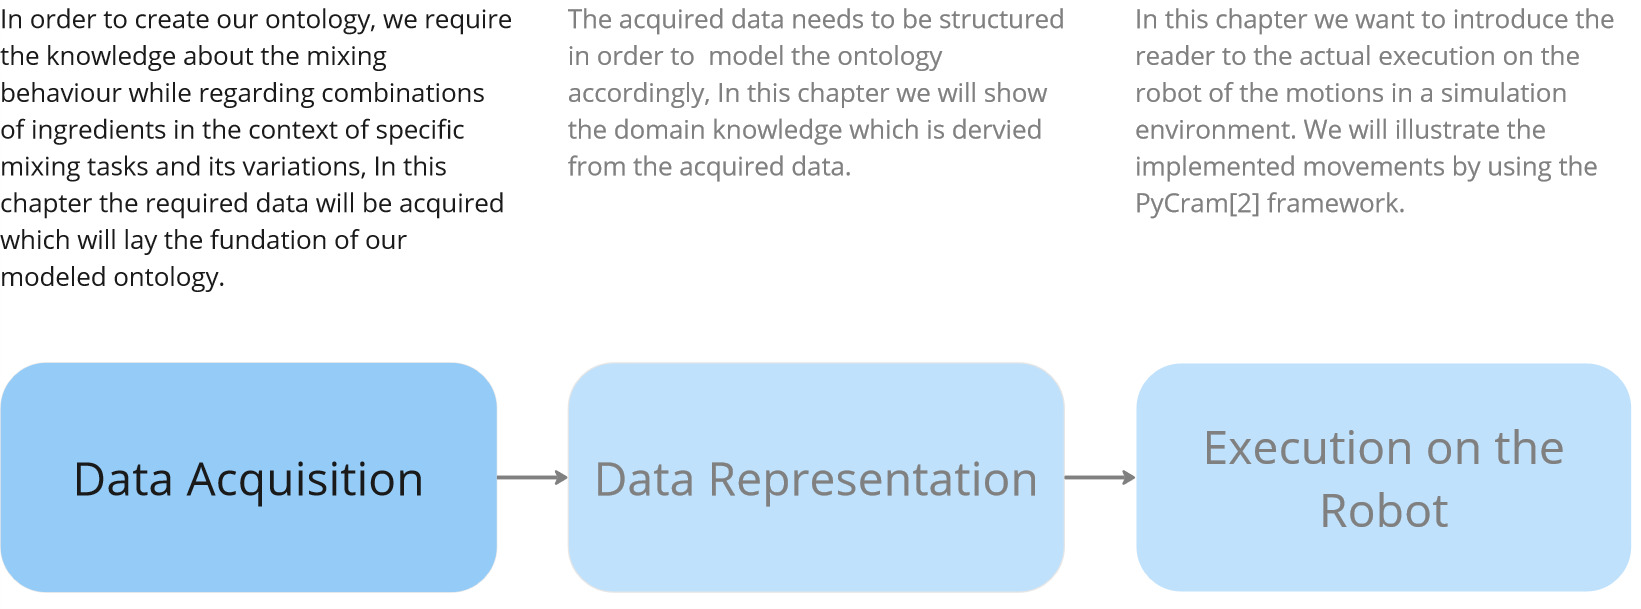
\includegraphics[scale=0.25]{Graphics/structure_overview1.jpg}
  \caption{Structure Overview: \textit{Data Acquisition}}
\end{figure}
Data acquisition involves understanding what mixing is, how it is performed by people, and how connections can be derived from video analyses. Essentially, it’s about discovering the various ways mixing is done, the contexts in which it occurs, and what insights we can draw from it. This includes identifying different mixing motions, determining which contexts are relevant, and which can be disregarded.
First we have to ask ourselves for our context \textbf{What is Mixing?}
\paragraph*{What is Mixing?}
  The definition provided by the Oxford Dictionary \cite{Oxford} is as follows:
  
  \textbf{Definition:} To put together or combine (two or more substances or things) so that the constituents or particles of each are interspersed or diffused more or less evenly among those of the rest; to unite (one or more substances or things) in this manner with another or others; to make a mixture of, to mingle, blend.

  Ultimately, this definition conveys that mixing requires at least two elements or substances, which are then combined (evenly) with each other, resulting in a (new) substance.
  This definition is general and can be applied to various contexts. For our work, the aspect of cooking or mixing different (cooking) ingredients is important. Therefore, we consider some hyponyms of the verb \textit{Mixing} irrelevant for our cause and do not take them into account.
  An adapted definition for our work could be: 
  
  \textbf{Definition:} \textit{Mixing} is the combination of various (cooking) ingredients through different motions in a container.
  

\section{Task variations}
Now that we have defined what \textit{Mixing} means in our context, we aim to identify the various types of \textit{Mixing} and determine which ones are important for our work. We will also specify which types of \textit{Mixing} we will not consider further, providing arguments for our decisions.
	As our main focus is to represent the knowledge about mixing, first we had to acquire the different types and variations of mixing in order to create a complete Knowldegerepresentation. The first step in acquiring the needed data, was to acknowledge which task varations of mixing are actually important. 
  So we had to analyze the word \textit{Mixing} and its hyponyms. 
\subsection{Hyponyms} 
	Hyponyms are subordered words of a given word, for example one hyponym of \textit{Mixing} could be \textit{Beating}\cite{oxford_hyponym}.
  To conduct this analysis, one can utilize tools from various websites, such as FrameNet\cite{FrameNet} and WordNet\cite{WordNet}. These platforms provide users with the ability to search for specific words and obtain various associations for those words, including synonyms, acronyms, or, crucial for our case, hyponyms.	
  A full list of the considered hyponyms can be seen in table \ref{tab:hyponyms}.
\subsubsection{WikiHow Extraction}
  For all those hyponyms, we delegated a \textit{WikiHow} extraction search (see:\nameref{sec:WikiHow}) which should show us, how many times one of these words occur, in the context of cooking.
	To execute the search, we define a new Class \textit{MixingVerb}, which represents the verb \textit{Mixing} and its hyponyms.
  
  For the search, we consider each verb and a triple consisting of the verb forms. We consider three forms of the verbs: the infinitive, the past tense, and the present progressive. An example of such a search would be:
  \begin{lstlisting}
      MIX ("mix", "mixed", "mixing")
  \end{lstlisting}

    After we have defined the desired verbs that we ultimately want to search for, we want to adjust some search parameters. The crucial parameters involve filtering the categories; in our case, we want to focus on mixing in the cooking domain. Therefore, we filter out all articles that do not exist in the \textit{Food and Entertaining} category.
  \subsubsection{Hyponyms Occurance}
    For each defined verb, a search is initiated to determine how often this verb appears in the \textit{WikiHow} \cite{wikihow} articles. This is done to ascertain which verbs are ultimately relevant for our implementation and which ones we can exclude, as they are infrequently used in everyday language.
    In the table below the results can be seen.
    \begin{table}[H]
        \centering
        \begin{tabular}{|c|c|}
          \hline
          \textbf{Hyponym} & \textbf{Occurance}  \\
          \hline
          Mix & 5300 \\
          \hline
          Amalgamate & 0 \\
          \hline
          Beat & 956 \\
          \hline
          Blend & 1041 \\
          \hline
          Coalesce & 1 \\
          \hline
          Combining & 3591  \\
          \hline
          Coommingle & 0 \\
          \hline
          Compound & 0 \\
          \hline
          Conflate & 0 \\
          \hline
          Folding & 821 \\
          \hline
          Fuse & 17 \\
          \hline
          Intermix & 0 \\
          \hline
          Join & 53 \\
          \hline
          Jumble & 0 \\
          \hline
          Lump & 7 \\
          \hline
          Merge & 6 \\
          \hline
          Pair & 352 \\
          \hline
          Stir & 6027 \\
          \hline
          Unify & 2 \\
          \hline
          Unite & 2 \\
          \hline
          Whip & 863 \\
          \hline
          Whisk & 2267 \\
          \hline
          
    
        \end{tabular}
        \caption{\textit{Mix}-verb synoyms/hyponyms occurance}
        \label{tab:hyponyms}
      \end{table}
      
  \subsubsection{Further Examination and Conclusion}
  This search is ultimately intended to provide us with information on which tasks we want to represent in the knowledge base. Therefore, we decide on certain tasks based on two conditions: frequency and executability. The first condition is easy to understand; tasks that do not occur or occur very rarely are not considered. The second condition relates to the executability of the task in the context of robot movements. Additionally, some tasks with relatively high frequency are also examined more closely, as in English, the past tense is used as an adjective under certain circumstances.

Taking into account the first condition, the following tasks are not considered: \textit{Amalgamate, Coalesce, Comingle, Compound, Conflate, Fuse, Intermix, Join, Jumble, Lump, Merge, Unify, and Unite}.

The second condition excludes another task: \textit{Blend. Blend} is mostly used in the context of a blending machine, which is not handled by the robot. Without this machine, the blending execution cannot be performed correctly, so this task is excluded for us.

Upon closer examination, we will also not consider the verb \textit{Whip} because it is mostly used as an adjective for ingredients, such as whipped cream. This highlights that only the verb \textit{Whip} has relatively low frequency. The same applies to \textit{Pair}, where the past tense is used to describe a combination of different ingredients, such as wine paired with cheese.

The verb \textit{Combine} is not informative regarding the executed movement of an action and is equated to the verb \textit{Mix}.

Thus, the tasks we consider are: \textit{Mix, Beat, Fold, Stir, and Whisk.}

\section{Task Analysis and Defintion}
\label{sec:task_analysis}
Now that we have selected the tasks, they need to be analyzed to understand the context in which they are ultimately used. 
Our goal is for the robot to perform these tasks in a manner similar to how a human would. 
To achieve this, in the next step, we need to closely examine these tasks. 
It is recommended to analyze videos on \textit{WikiHow} \cite{wikihow} or other sources where these tasks are presented as activities. 
The analysis involves observing the movements associated with each task. 
We present these analyses in tabular form below. The examination includes the task itself, the respective ingredients being processed, the tools used for it, and the container in which the task is carried out.
The tasks will be ennumerated, and we will provide the full table with the actual video source in the \nameref{chap:appendix}.
    \begin{table}[H]
    \centering
    \begin{tabular}{|c|p{5,5cm}|p{6,5cm}|}
        \hline
        \textbf{Task} &  \textbf{Ingredients} & \textbf{Description} \\
        \hline
        Beating &  Egg yolk & circular, swirling wildly around the bowl \\
        \hline
        Stirring & Beaten Egg Yolk , Parmesan and Pepper  & Circular, from the inside to the outside. \\
        \hline
        Whisk & Eggs  & Circular but also straight, wildly motion. \\
        \hline
        Mixing &  Eggs, melted butter & Circular, from the inside to the outside, also diving. \\
        \hline
        Folding & cooked eggs in melted butter & Gently motion from the outisde to the inside straight, then moving about 90 degree before going to the inside again. \\
        \hline
      \end{tabular}
    \caption{Video analysis}
    \label{tab:videoanalysis}
  \end{table}


After a thorough analysis of the videos and the information provided in them, we conclude that the executed movement is not only related to the task but also influenced by the ingredients used. However, some tasks are deterministic in the sense that the movement is performed regardless of the specific ingredients.

In the following, we aim to structure the extracted information from the videos and present our findings.

\subsection{Video Analysis Conclusion and Results}

Based on the extracted information, we conclude that for our goals, the following aspects, in addition to the task, are important and will be further considered:
\begin{itemize}
  \item \textbf{Ingredients}: The ingredients play a crucial role in the movement decision associated with the tasks and will be defined more precisely.
  \item \textbf{Tools}: The tools used may not be decisive in the movement decision. Since we do not consider electric tools, every motion can be performed with any tool.
  \item \textbf{Container}: As conducted with the tools, the container wont play a crucial in the motion decision. 
  \item \textbf{Motions}: The motions ultimately represent the movement of the robot for our implementation. These movements are extracted from the videos and defined in alignment with robot motions.
\end{itemize}

\subsubsection{Ingredients}
Through the video analysis , we come to the conclusion that the nature of ingredients is important. 
Primarily, ingredients can be divided into two main categories: \textit{Dry} and \textit{Wet} \cite{Ohene2017}. 
This division becomes crucial, especially regarding the measurement of quantities for each type of ingredient.

For our case, a somewhat finer categorization of ingredients is necessary to map the various movements sensibly to the given types. 
In addition to \textit{Wet} ingredients, we introduce 2 new sub-categories: \textit{Liquid} and \textit{Semi-Liquid} ingredients. 
This corresponds to ingredients falling under the \textit{Wet} ingredients but with a liquid or semi-liquid state, such as milk, water, eggs, butter and oil. 
This is significant because some movements differ when the given ingredients are \textit{Semi-Liquid} or \textit{Liquid}.

We will also include 2 sub-categories for the \textit{Dry} category, namely the \textit{Solid} and \textit{Powder} ingredients category. 
This differs from the each other in that it consists of solid components, while we define the \textit{Powder} category to include powdery substances. The \textit{Solid} category encompasses foods like vegetables, fruits, and meats. 
Through these distinctions, we can create a definition refining the ingredient categories.

Our initial set of ingredients is: \textit{Milk, Oil, Water, Vinegar, Vanilla Extract, Sauces}, \textit{Egg White, Egg yolk, Butter, Whipped Cream}, \textit{Flour, Salt, Sugar, Baking Soda, Cocoa Powder},
\textit{Onions, Pork, Chicken, Minced meat, Bacon}.

These ingredients are commonly used in the analyzed videos and are also very common ingredients for baking and cooking recipes.
In the chapter \nameref{chap:Data_representation} these classes will be categorized.

\subsubsection{Containers and Tools}
\label{sec:ContainersAndToolsAcquisition}
Throughout the analysis of \textit{WikiHow} videos common tools and containers were identied during the exuecution of various mixing tasks.
The most dominant occuring container was a bowl, followed by a pan, cup and then lastly a mug.
Those objects can be used to store and serve food for everyday meals. Thus these objects can be summarised 
into a single concept - \textit{Crockery} \cite{crockery}

Common occuring tools like a mixer, spatula, spoon and whisk were used. 
To acquire different kinds of tools and containers, we look into ontologies like \textit{SOMA-Home} \cite{soma},
where an hierarchy of containers and tools is defined. \textit{SOMA-Home} is a taxonomy modelling concepts for a kitchen environment. 
\textit{SOMA-Home} uses the class \textbf{Crockery}, the class of all kinds of containers.
Via subsumption over \textbf{Crockery}, we acquire different kinds of containers for mixing.

Identified tools from the video analysis are partially represented by \textit{SOMA-Home}, where mainly cutleries is defined in that ontology.
Some tools like mixers and whisks neither belong to the class of all cutleries nor are they represented in \textit{SOMA}. Retrieving a set of tools
for these exceptions can't be achieved.

To summarize, the following tools where identified: 
\begin{itemize}
  \item Cutlery
  \item Mixer
  \item Whisk
\end{itemize}

Containers are summarized into the concept of crockery. 
\subsubsection{Motions}
\label{sec:Motions}
From these videos, we extracted information about the executed motions. In this section, we will describe what the extracted motions are. 
Additionally, an abstract description is provided of how each motion is implemented in pycram2, using formulas and plots for visualization.
We hold the following assumptions about each motion:

\begin{itemize}
  \item Each container has a symmetric shape in the x and y directions, considering z as pointing either upwards or downwards.
  \item The height of the executed motion remains constant.
  \item There is no collision detection.
\end{itemize}

These motions were extracted during analysis of the videos:

\begin{enumerate}
  \item Circular Motion
  \item Folding Motion
  \item Horizontal Elliptical Motion
  \item Whirlstorm Motion
  \item Circular Diving To Inner Motion 
\end{enumerate}

\paragraph{Circular Motion}
The circular motion is generated on a circular plane, which effectively moves the tool in a circle. 
By having a center coordinate = $(centerX, centerY)$, which is the center coordinate of 
the container to execute the Circular Motion, we generate a set of coordinates
with the following functions: 

\[x = centerX + radius * cos(radian)\]
\[y = centerY + radius * sin(radian)\]

We retrieve the respective radians using the following function:

\[radian = angle * \frac{\pi}{180}\]

Generating a sequence of points lying inside a circle is accomplished by generating a sequence of angles starting from 0 to 360 degrees, 
converting them into radians, and using formulas to compute the circular coordinates.

\begin{figure}[H]
    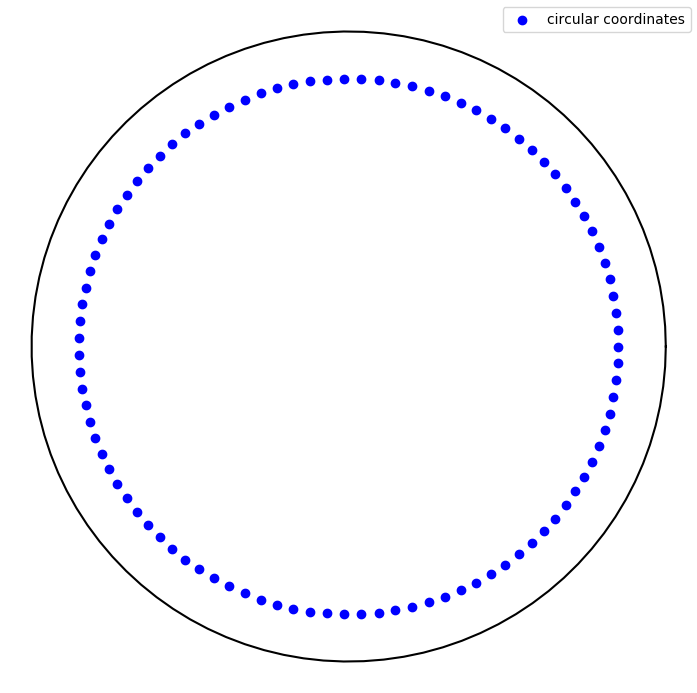
\includegraphics[scale=0.35]{Graphics/motions/circular_motion.png}
    \centering
    \label{fig:circularMotion}
    \caption{Top Down View - Circular Motion}
\end{figure}

\paragraph{Folding Motion}
The folding motion differs from circular motion; instead, it follows a linear trajectory.
This movement consists of lifting part of the ingredients and gently folding them over the rest.
A thorough mixing of the ingredients is possible because of this motion. Repetition of this method ensures even distribution throughout the mixture. 
It's a methodical and delicate approach to ingredient integration.
\newline
\newline
In its current implementation, the motion follows a singular line. One endpoint rests on the edge of the container, while the other is positioned at the center.
Although the motion itself is a straight line traversing the container, it is executed by moving from one end to the center and then repeating 
the motion in reverse—from the center to one of the ends, creating a folding effect.
While this line covers only part of the container, its direction needs realignment to mix different sections of the container thoroughly

This can be accomplished by a 2D transformation, constructing a 2D rotation matrix for some angle $\theta$, where $\theta$ determines the rotation of the line.
\[R(\theta) = \begin{bmatrix}
    \cos(\theta) & -\sin(\theta) \\
    \sin(\theta) & \cos(\theta)
     \end{bmatrix}
 \] 

and applying the transformation to the line using this function:

\[\begin{bmatrix} x' \\ y' \end{bmatrix} = R(\theta) * \begin{bmatrix} x \\ y \end{bmatrix}\]

\begin{figure}[H]
    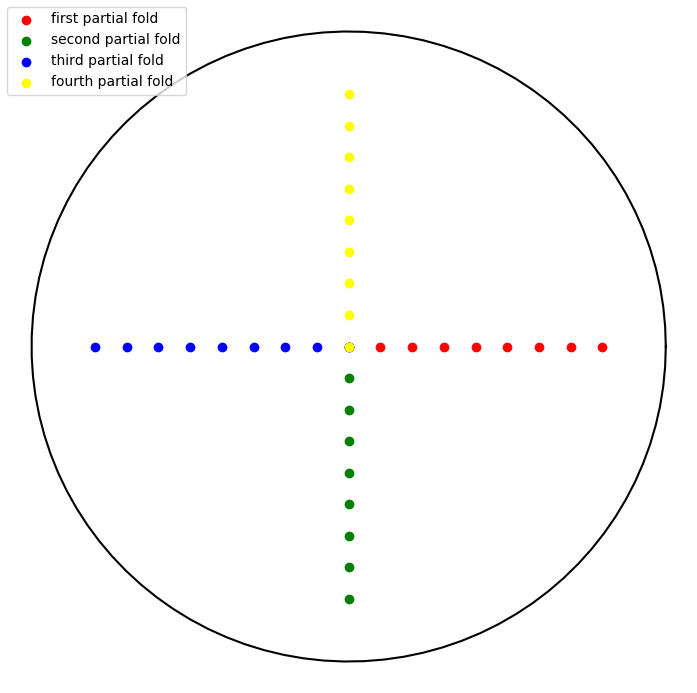
\includegraphics[scale=0.35]{Graphics/motions/folding0.png}
    \centering
    \label{fig:foldingMotion1}
    \caption{Top Down View - Folding 4 areas of a container}
\end{figure}

In this example, the folding motion is applied to four different sections of the circular container.
The number of areas covered or the angle at which the folding line is adjusted is not critical.
The fundamental movement remains consistent: the motion proceeds along a line and then reverses."

After executing the folding motion to cover various parts of the container, we apply a transformation with a different angle $\phi$.

\begin{figure}[H]
    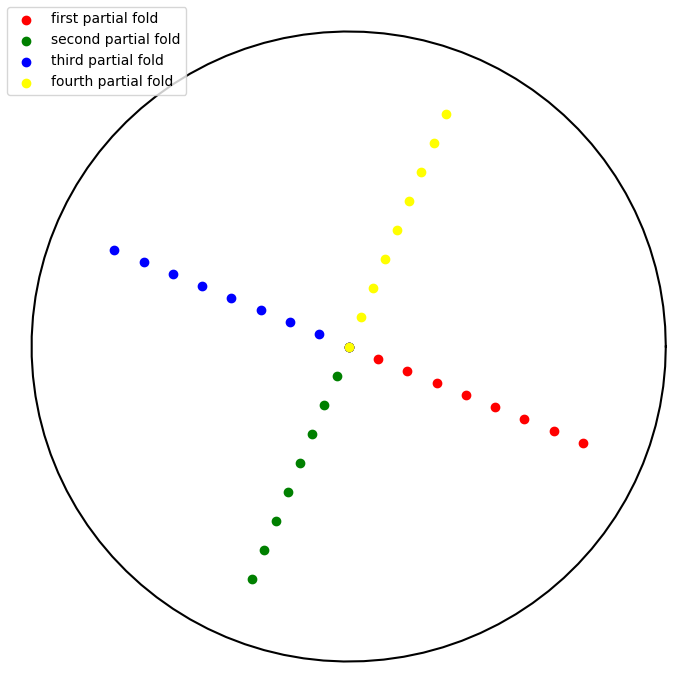
\includegraphics[scale=0.35]{Graphics/motions/folding1.png}
    \centering
    \label{fig:foldingMotion1}
    \caption{Cover different areas of the container with $\phi=22.5$}
\end{figure}

\paragraph{Horizontal Elliptic Motion}
The horizontal elliptic motion is executed on a horizontal plane and involves multiple ellipses to cover the entire container.
This motion is commonly employed in the task of beating, where ingredients within a container are thoroughly mixed through stirring or beating.
\newline
\newline
Using the function to compute x,y coordinates on a circle, we use two different radii.
One radius is a small value, whether it is an absolute value or relative to the dimensions of the container. The other radius is sampled from an interval. 
The interval is defined as \[radii = [radius, \frac{radius} {2} ]\]
meaning the sampled radius ranges from the full radius of the container to half of that radius.

A sampled radius from this interval is taken, if the following condition is true for all resulting circle coordinates:
\[\sqrt{(xCord - xCenter)^2 + (yCord - yCenter)^2} < radius\] 

The end result will be ellipses that are narrow on one axis and conform to the shape of the container on the other axis.
A generated ellipse considering the above conditions can look like this:

\begin{figure}[H]
    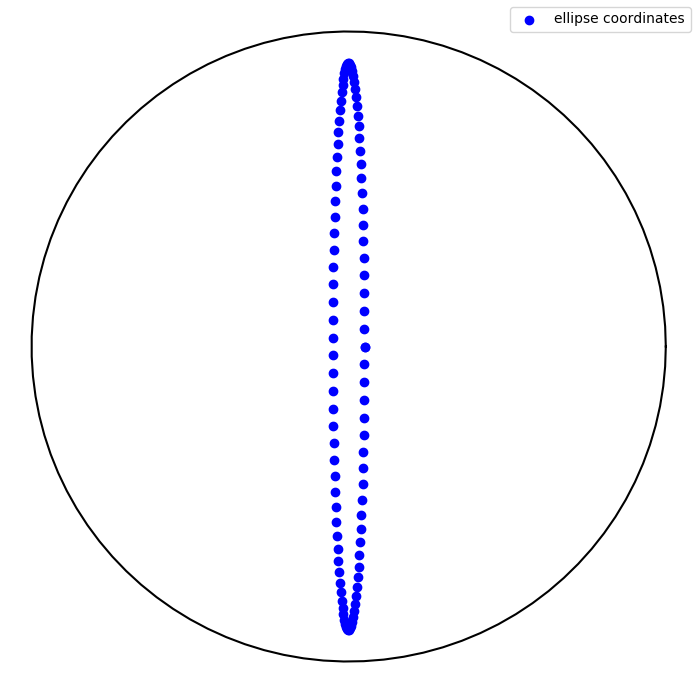
\includegraphics[scale=0.35]{Graphics/motions/ellipse.png}
    \centering
    \label{fig:foldingMotion1}
    \caption{Top Down View - Single Ellipse}
\end{figure}


To cover most areas of any container and assuming that generating y-coordinates used a constant radius, all y-coordinates are shifted after generating the ellipses. 
To check if the y-coordinates are within the container's bounds, the following condition is checked for every y-coordinate:

\[\sqrt{(yCord)^2 + (yCenter)^2} < radius\]

If this condition is met, the direction of the shift is reversed, switching from incrementing to decrementing and vice versa.

One horizontal elliptic motion consisting of multiple ellipses could look like this:

\begin{figure}[H]
    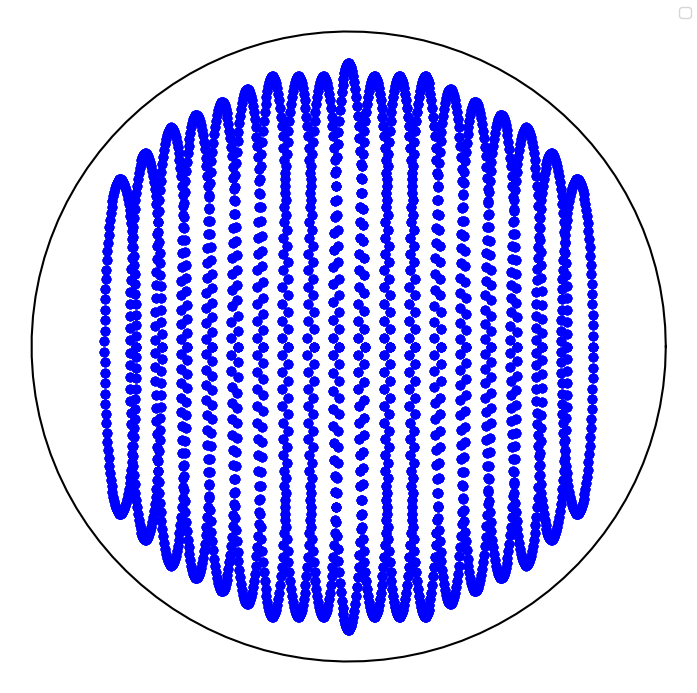
\includegraphics[scale=0.35]{Graphics/motions/horizontal_elliptical.png}
    \centering
    \label{fig:foldingMotion1}
    \caption{Multiple ellipses covering the containers area}
\end{figure}


\paragraph{Whirlstorm Motion}
The whirlstorm motion uses the function to generate circle coordinates  with differing radii sampled from an interval:
\[[upperBoundRadius, lowerBoundRadius]\]

\begin{figure}[H]
    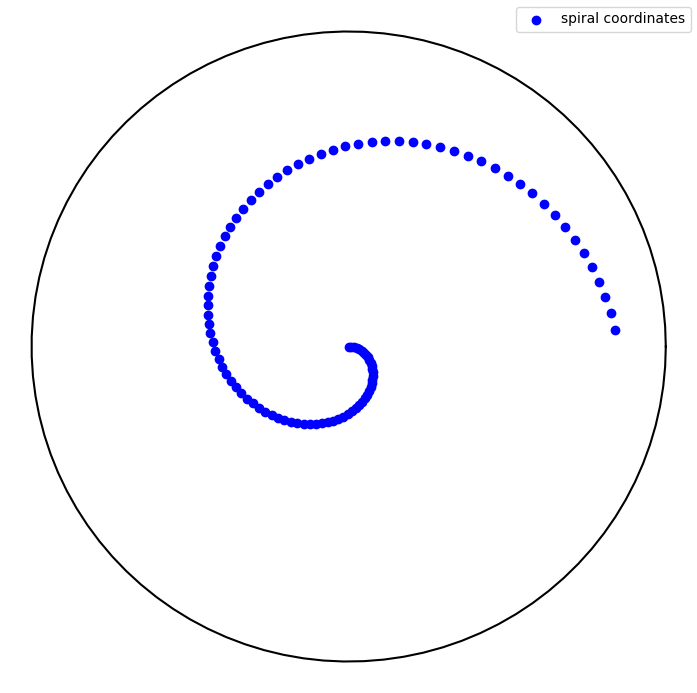
\includegraphics[scale=0.35]{Graphics/motions/whirlstorm1.png}
    \centering
    \label{fig:foldingMotion1}
    \caption{Multiple ellipses covering the containers area}
\end{figure}


The whirlstorm motion is a dynamic and complex swirling pattern that simulates a series of interconnected spiral motions. 
This motion starts outwardly gradually moving to the inner part of a container, creating a visual effect reminiscent of a whirlpool or tornado. 
The movement alternates in direction and shape periodically, ensuring a diverse and comprehensive coverage within the containers bounds.
This results in a fluid, spiraling trajectory, effectively mimicking natural swirling motions.

In total four whirlstorm patterns are generated, where the first two pattern look like this:

\begin{figure}[H]
    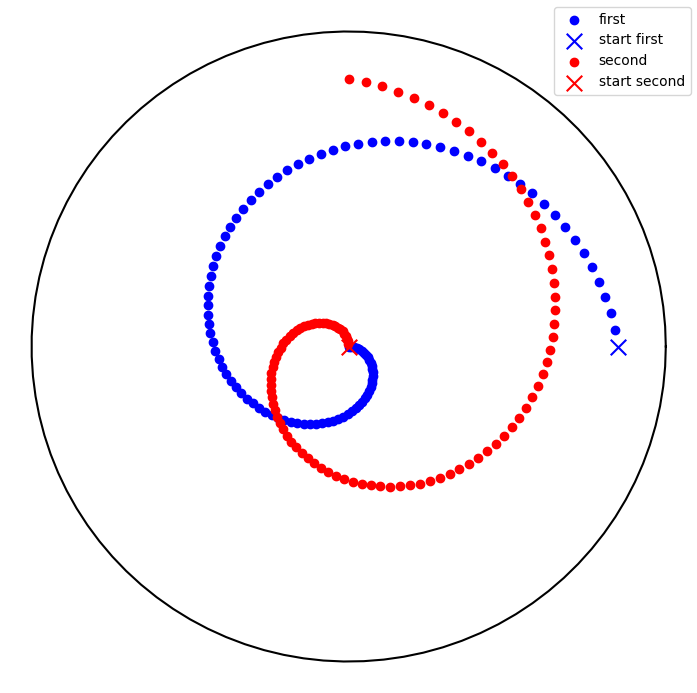
\includegraphics[scale=0.35]{Graphics/motions/whirlstorm2.png}
    \centering
    \label{fig:foldingMotion1}
    \caption{Multiple ellipses covering the containers area}
\end{figure}
The third and fourth look like this:

\begin{figure}[H]
    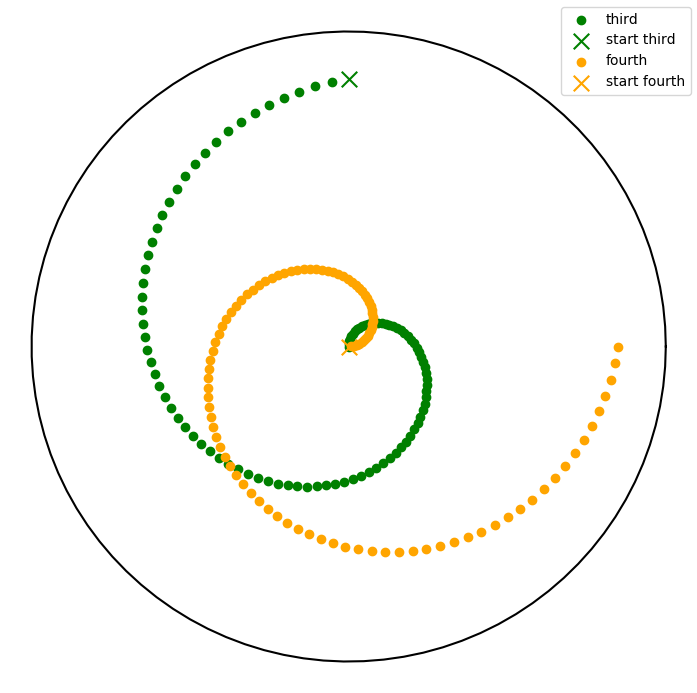
\includegraphics[scale=0.35]{Graphics/motions/whirlstorm3.png}
    \centering
    \label{fig:foldingMotion1}
    \caption{Multiple ellipses covering the containers area}
\end{figure}

\paragraph{Circular Diving To Inner}
This motion is a circular motion, where the tool is dipped into the container, causing the ingredients to be stirred up and down.
This creates a consistent mixture. However, since dipping is involved, 
which directly contradicts our assumption that height remains constant over the course of the motion, and eventually leaves the boundaries of the used container, 
we don't provide an abstract implementation of this motion. This motion will have a representation in our \textit{mixing} ontology but won't be implemented in pycram2.


\section{Data Acquisition Conclusion}
The data acquisition lays the foundation to create a model, mainly an \textit{OWL} ontology, to define relationships between the identified actors for various mixing tasks.
By identifying several tasks which were executed in the \textit{WikiHow} videos \cite{wikihow}, we were able to define specific motions from different 
kinds of mixing tasks. 

The motions that need to be executed are heavily dependent on the task and the set of ingredients used for mixing.
Tools and containers are more or less negligible for the execution of the motions. 
However, they are still considered, since each container can store different kinds of food, and tools are limited to the container being used.

In total five different motions were identified, which will be executed onto four subcategories of ingredients. 
In the following chapter we will present a taxonomy of mixing with all relevant actors, which enables the robot to execute various mixing tasks in simulation. 
\newpage